\documentclass[11pt]{article}
\usepackage[margin=2.5cm]{geometry}
\usepackage{graphicx}
\usepackage{booktabs}
\usepackage{amsmath}
\usepackage{amssymb}
\usepackage{parskip}
\usepackage{enumitem}
\usepackage[colorlinks=true,linkcolor=blue,citecolor=blue]{hyperref}

\title{Paper 1 Progress Update: BLG vs. $\beta$-Casein at the Air--Water Interface}
\author{Chalakon Pornjariyawatch \\ COMFHA Lab, Kasetsart University}
\date{September 25, 2026}

\begin{document}
\maketitle

\noindent\textbf{Prepared for:} Prapasiri Pongprayoon (P.P.) \\
\textbf{Purpose:} Status update on the comparative BLG/$\beta$-casein adsorption study --
results and open questions since the last update (September 11, 2026).

\section*{Executive Summary}
\noindent\textit{Changes since the last update (September 11, 2026):}
\begin{itemize}[itemsep=2pt]
  \item \textbf{The BLG data-completeness gap flagged in the last update is half closed.}
    $R_g$ for R1/R2/R3 now covers the full 1000 ns per replica (fixed today --
    \texttt{blg\_rg.py}'s trajectory-extension gap is closed). Surface tension for those
    same three replicas still reflects only the first 500 ns; the extension segments'
    \texttt{.edr} energy files exist on the cluster but have not yet been synced locally,
    so that fix is still pending.
  \item \textbf{Structural renders (Figure~\ref{fig:schematic}) rebuilt at full
    publication resolution.} The previous report's calyx/N-term renders were a stale
    512$\times$512 px placeholder (headless VMD's default framebuffer size); regenerated
    today at 3008$\times$2400 px, and the figure now also includes the simulation box
    geometry panel.
  \item No change to the core scientific picture: BLG remains stable and compact across
    all 4 replicas, and CASEIN's two-replica comparative result (open, persistently
    surface-exposed N-terminus vs. BLG's small, selectively-accessible calyx) --
    reported in full in the September 11 update -- still holds with no new data since.
  \item \textbf{5 open questions remain for P.P.} (Section~\ref{sec:questions}), unchanged
    since the June 9 meeting -- none carry a hard deadline, but two now block downstream
    figure/writing decisions.
\end{itemize}

\section{Structural Overview}

Figure~\ref{fig:schematic} re-renders both proteins' key accessible feature at full
publication resolution (VMD structural renders regenerated today at 3008$\times$2400 px,
up from a stale 512$\times$512 px render -- headless VMD's default framebuffer size,
fixed via the \texttt{-size} launch flag rather than an in-script resize, which crashes
in text-mode VMD) alongside the simulation box geometry for each species.

\begin{figure}[h]
\centering
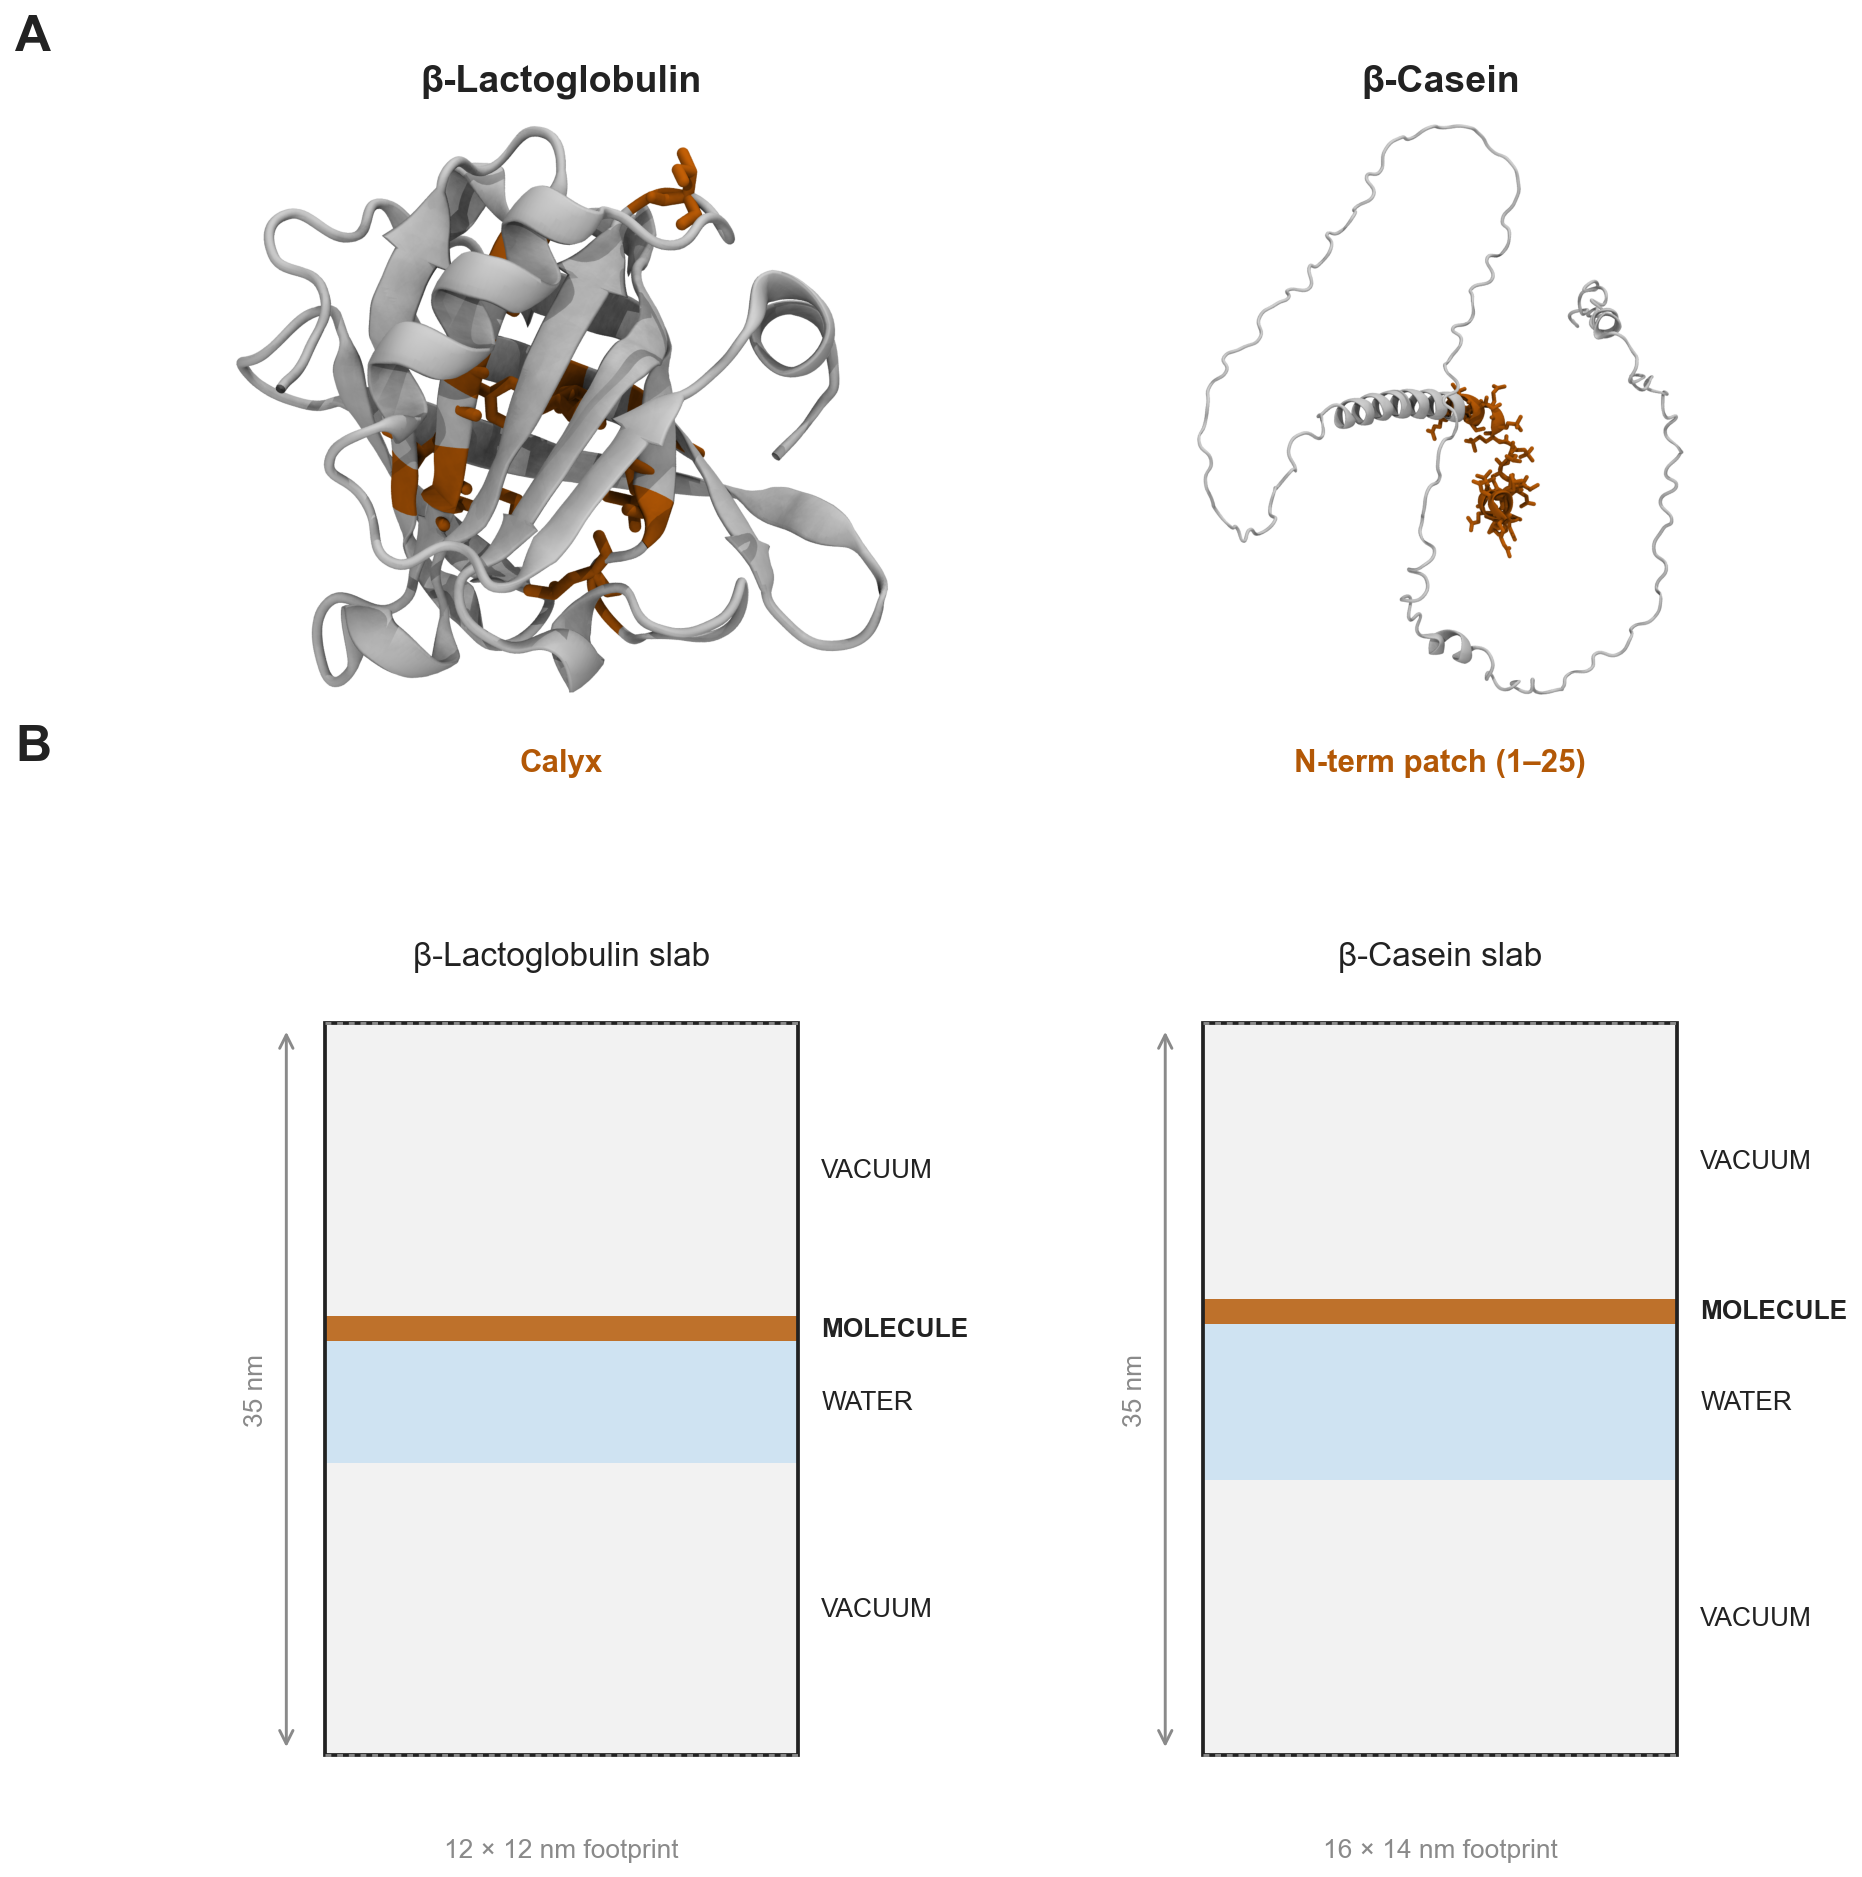
\includegraphics[width=\textwidth]{../results/figures/paper/PAPER_FIG1_SCHEMATIC.png}
\caption{(A) BLG's calyx (9 lining residues, amber) versus CAS's N-terminal
accessible patch (residues 1--25, amber), both rendered at the same visual
convention (NewCartoon, ambient occlusion, orthographic). (B) Slab simulation box
geometry for each species, drawn to the real locked box dimensions.}
\label{fig:schematic}
\end{figure}

\section{BLG Results}

BLG's headline numbers are unchanged from the last update and remain fully validated
across all 4 replicas (CENTER + R1/R2/R3, 4.00~$\mu$s total unbiased MD).

\begin{table}[h]
\centering
\small
\begin{tabular}{lcccc}
\toprule
Replica & Calyx SASA (nm$^2$) & $R_g$ (nm) & $\gamma$ (mN/m) & Patch RMSD (nm) \\
\midrule
CENTER (1000 ns) & 3.81 $\pm$ 0.46 & 1.504 $\pm$ 0.022 & 51.9 $\pm$ 38.5 & 0.198 $\pm$ 0.081 \\
R1                & 3.15 $\pm$ 0.34 & 1.497 $\pm$ 0.009 & 52.7 $\pm$ 38.7* & 0.347 $\pm$ 0.088 \\
R2                & 3.59 $\pm$ 0.32 & 1.494 $\pm$ 0.009 & 52.0 $\pm$ 39.0* & 0.254 $\pm$ 0.059 \\
R3                & 3.36 $\pm$ 0.48 & 1.507 $\pm$ 0.014 & 52.6 $\pm$ 39.4* & 0.276 $\pm$ 0.064 \\
\bottomrule
\end{tabular}
\caption{BLG per-replica summary. $R_g$ for R1/R2/R3 now covers the full 1000 ns
(\texttt{blg\_rg.py}'s trajectory-extension gap was closed today, 2026-09-25). *$\gamma$
for R1/R2/R3 is still computed from the first 500 of 1000 ns per replica --
\texttt{blg\_surface\_tension.py} needs the extension segments' \texttt{.edr} energy
files, which exist on the cluster but have not yet been synced locally. Not expected
to change the qualitative picture, but not yet closed out.}
\end{table}

The calyx stays compact and accessible in every replica (no collapse), Rg confirms a
globally stable fold, and 613 discrete contact events occur across the full dataset
with zero sustained (``gate-open'') adsorption events -- the basis for the paper's
scope claim (pre-commitment characterisation, not a completed-adsorption mechanism).
R1's elevated patch RMSD (0.347 nm vs. 0.20--0.28 nm in the other three) is a real,
traced effect: R1 contains 4 of the project's 6 total long ($\geq$10 ns) contact
events, and the patch RMSD steps up permanently after its longest event
(362--419.5 ns) without ever returning to baseline -- a genuine local
conformational response to sustained contact, not noise.

\begin{figure}[h]
\centering
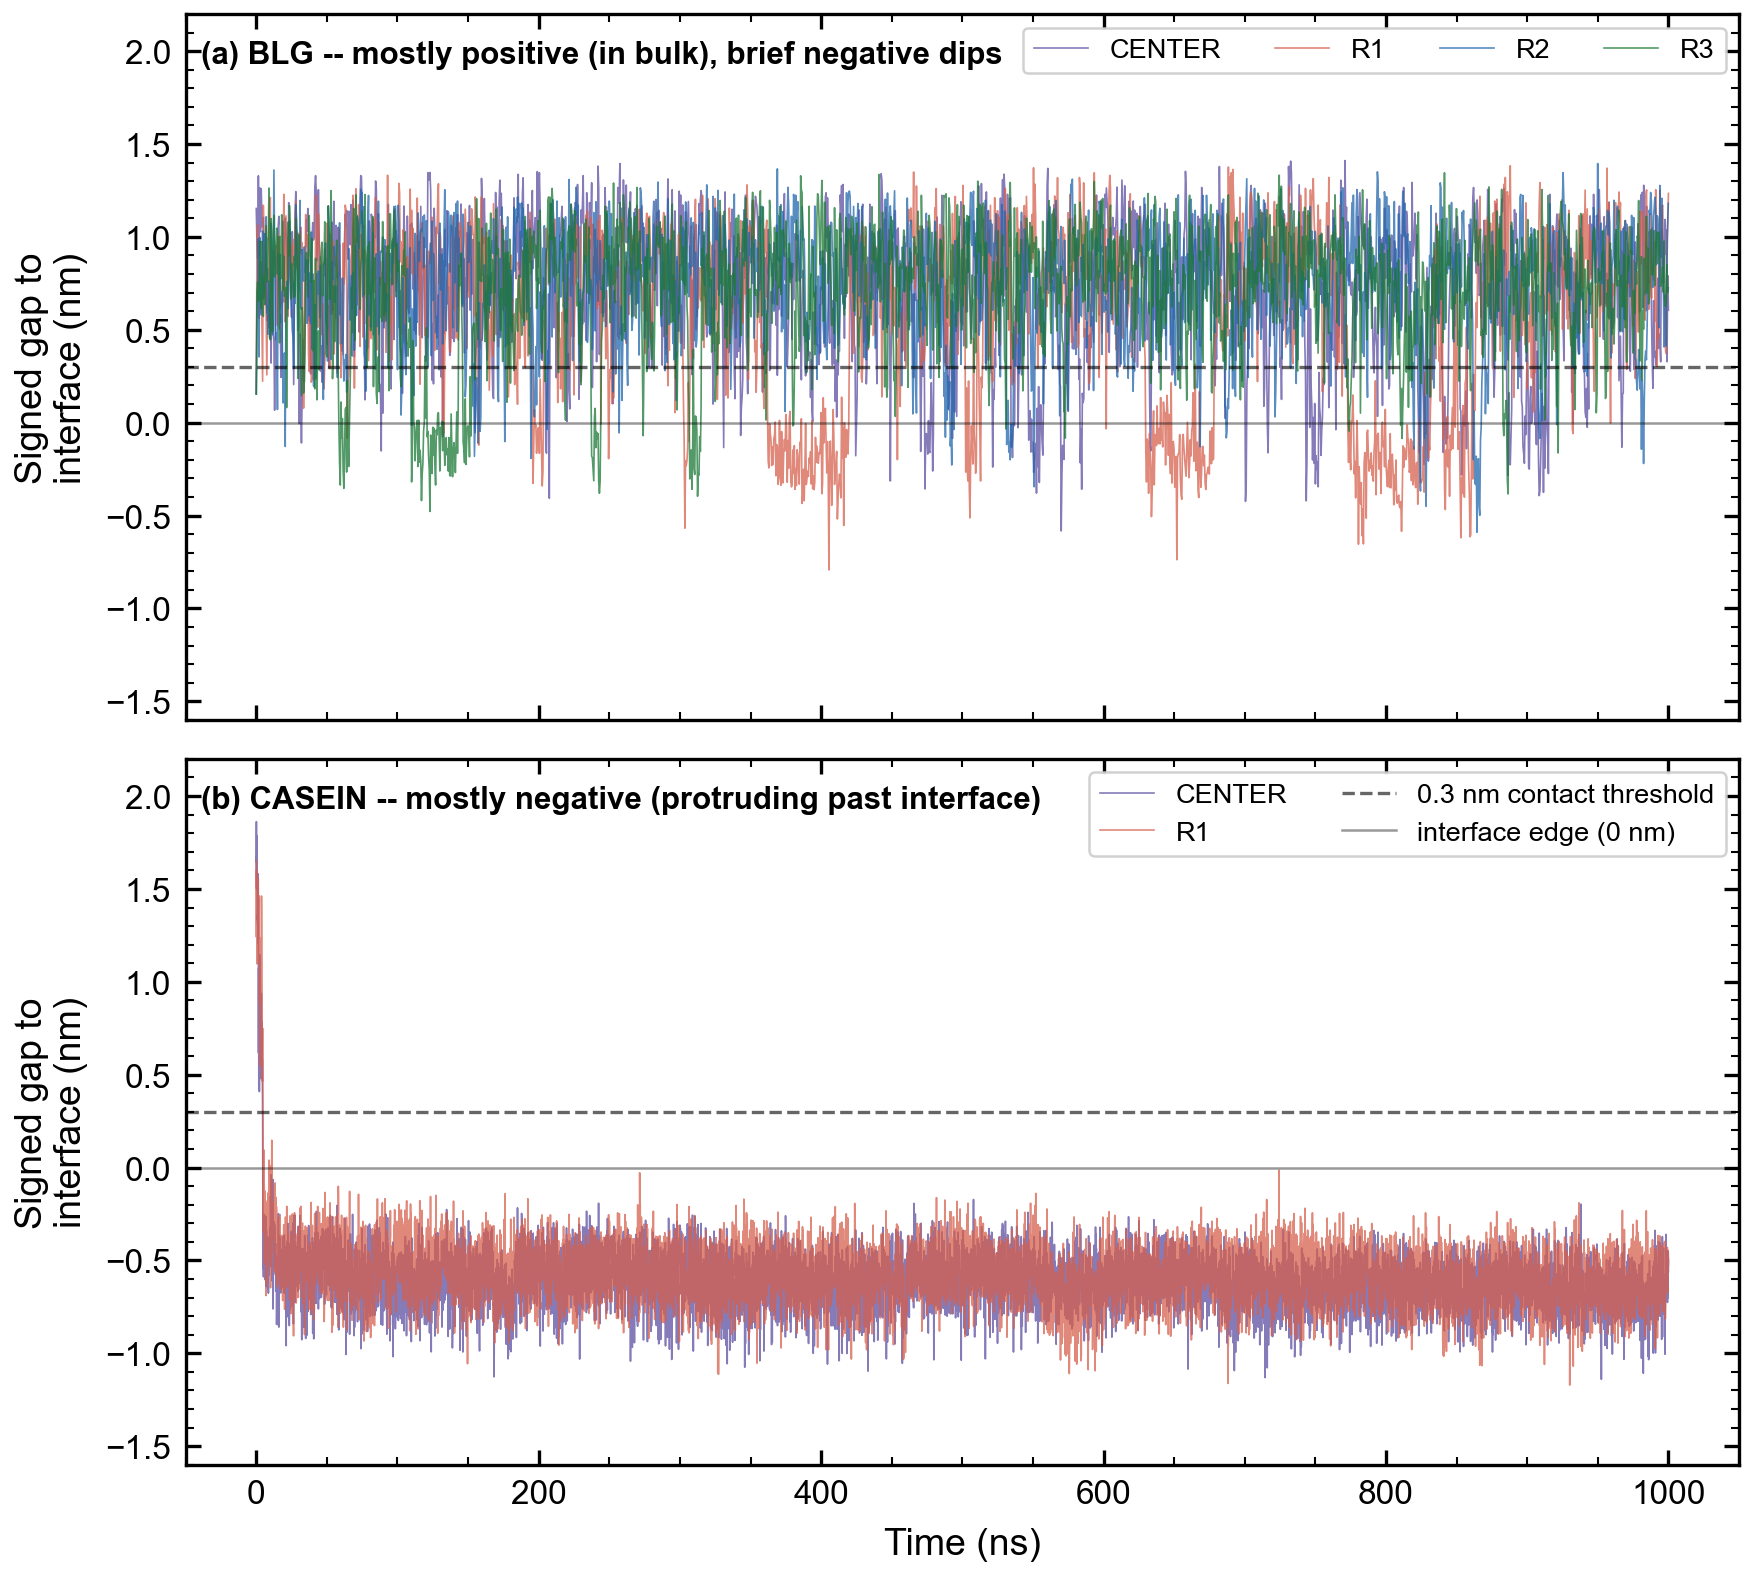
\includegraphics[width=0.78\textwidth]{../results/figures/paper/PAPER_TIMESERIES_CONTACT.png}
\caption{Signed protein-to-interface gap vs. time (positive = inside the water bulk,
negative = protruding past the interface). BLG sits mostly positive with brief,
distinct negative excursions -- its 613 contact events.}
\end{figure}

\section{$\beta$-Casein (CAS) Results}

\textbf{7 of 7 planned analyses complete, now for both CENTER and R1} -- the first
time every CAS headline metric has independent-replica confirmation rather than a
single run.

\begin{table}[h]
\centering
\small
\begin{tabular}{lccccc}
\toprule
Replica & N-term SASA (nm$^2$) & Contact & $\gamma$ (mN/m) & Hbonds prot-prot & Hbonds prot-water \\
\midrule
CENTER (1000 ns) & 25.41 $\pm$ 1.97 & 99.5\% & 51.4 $\pm$ 34.2 & 97.8 $\pm$ 9.7 & 565.5 $\pm$ 25.1 \\
R1 (1000 ns)     & 24.77 $\pm$ 1.40 & 99.5\% & 52.4 $\pm$ 34.6 & 92.0 $\pm$ 8.3 & 575.9 $\pm$ 24.0 \\
\bottomrule
\end{tabular}
\caption{CAS per-replica summary. ``Contact'' is the fraction of frames with a
protein-water minimum distance $\leq$0.3 nm; each replica shows 1 sustained contact
event across the full 1000 ns run.}
\end{table}

CAS's N-terminal region (residues 1--25, the analogue of BLG's calyx) stays large and
accessible in both replicas -- a $\sim$7-fold size difference from BLG's calyx that
holds at every timepoint, not just on average. Rg confirms the same relaxation
pattern in both replicas: an initial compaction from the extended AlphaFold starting
structure ($\sim$2.85 nm, first $\sim$100 ns) settling to a stable range
($\sim$2.5--2.7 nm) for the remainder of the trajectory -- a real, reproducible
relaxation transient, not a one-off artifact of either run's starting conformation.
Hydrogen-bonding agrees closely between replicas (protein-protein 92.0--97.8,
protein-water 565.5--575.9, interface water-water 12015.6--12750.5 mean counts per
frame).

\begin{figure}[h]
\centering
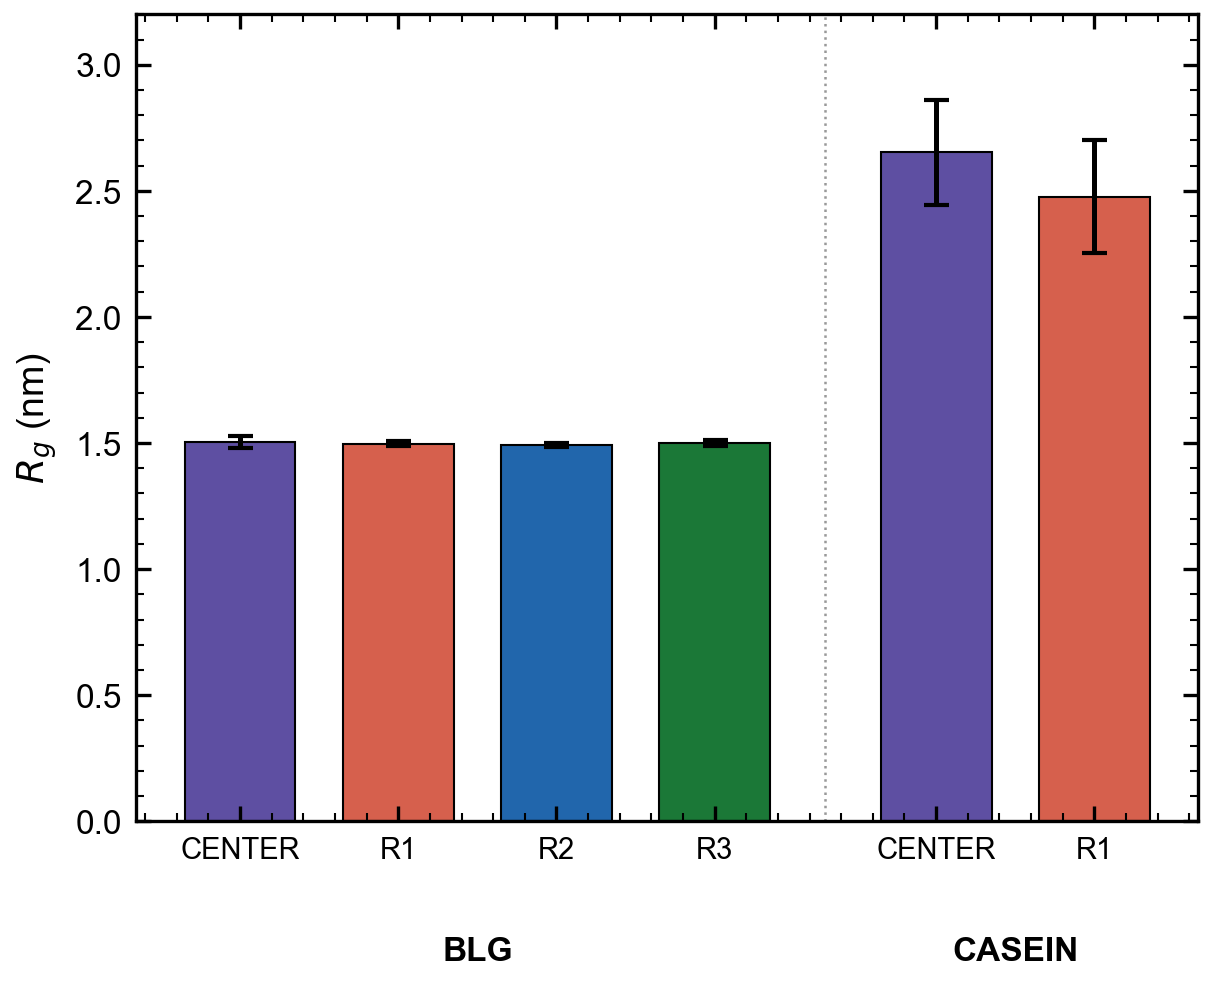
\includegraphics[width=0.6\textwidth]{../results/figures/paper/PAPER_COMPARATIVE_RG.png}
\caption{Radius of gyration, BLG vs. CAS, all replicas. BLG stays tightly compact
($\sim$1.5 nm) while CAS settles to a larger, stable range ($\sim$2.5--2.7 nm) after
its initial relaxation.}
\end{figure}

\begin{figure}[h]
\centering
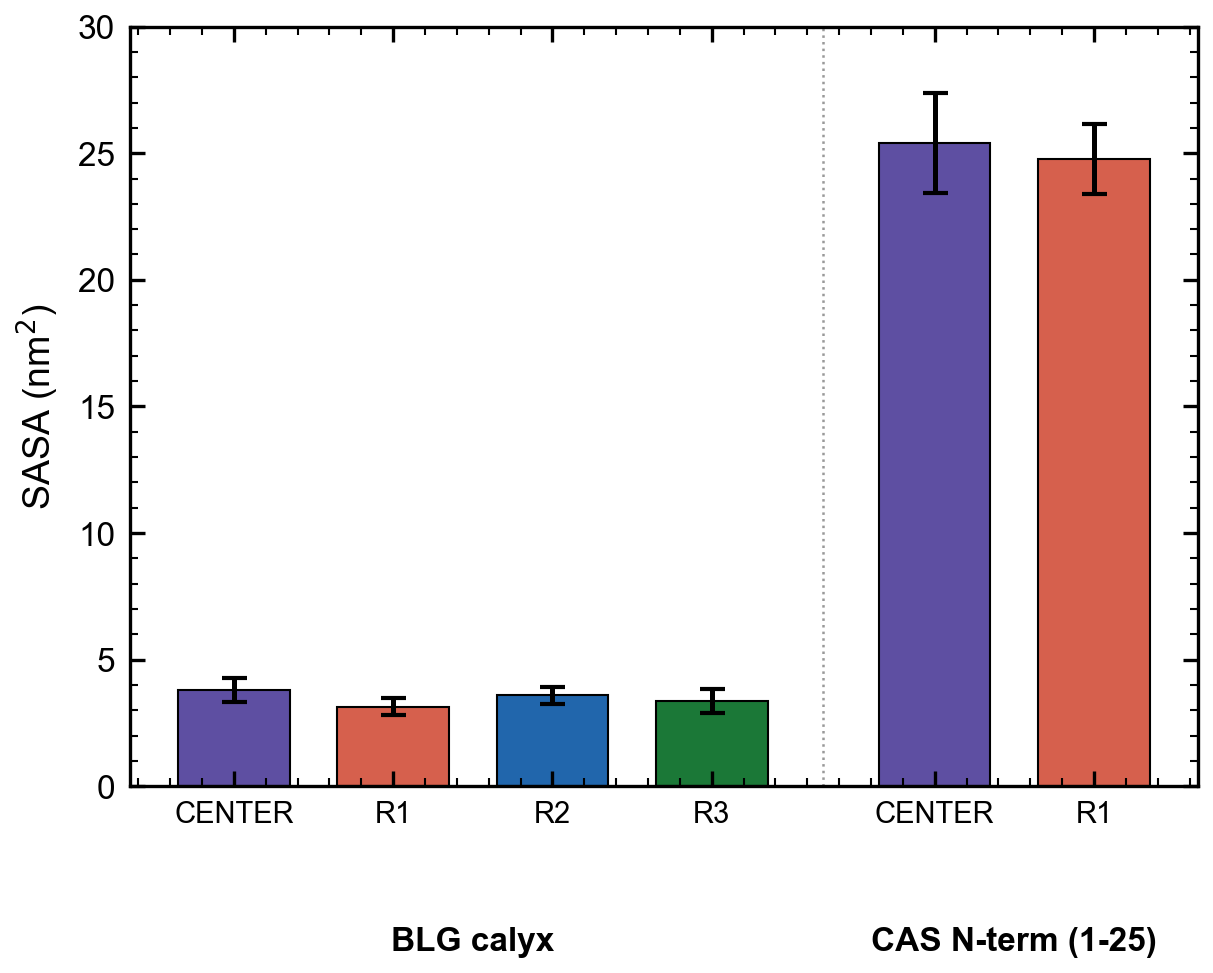
\includegraphics[width=0.78\textwidth]{../results/figures/paper/PAPER_COMPARATIVE_SASA.png}
\caption{Accessible surface area, BLG calyx vs. CAS N-terminal region, all replicas.
The $\sim$7-fold size difference is consistent across every replica of both proteins.}
\end{figure}

CAS's near-constant interfacial contact (99.5\% of frames, both replicas) versus
BLG's selective, intermittent contact pattern is the clear structural contrast that
directly supports the comparative title: BLG presents a small, selectively-accessible
calyx, while CAS's disordered chain stays persistently near the interface with its
N-terminal region continuously exposed.

\section{Questions for P.P.}
\label{sec:questions}

Full detail for all items below is tracked in \texttt{docs/PP\_FEEDBACK\_LOG.md}. No
item carries a near-term (\textless 30 day) deadline; the list is unchanged since the
June 9 meeting.

\begin{enumerate}[itemsep=4pt]
  \item \textbf{Secondary-SASA definition.} Your note ``secondary dasa'' from the June
    9 meeting is ambiguous. Our best reading: absolute SASA computed per
    secondary-structure element (DSSP region $\times$ SASA) -- computable now. A
    $\Delta$SASA-on-adsorption reading is \emph{not} computable, since no completed
    adsorption event exists in either dataset. Please confirm which you meant.
  \item \textbf{Which lab experiments to correlate against?} Your note said
    ``correlation with lab experiment expected.'' We see no in-house
    tensiometry/Langmuir-trough data in the repo, so we've assumed you mean published
    literature (already surveyed: Cornec 1999, Ulaganathan 2017a for BLG kinetics;
    Mackie 1999 for CAS rheology; Atkinson 1995 for CAS N-terminal neutron
    reflectivity). Please confirm this reading.
  \item \textbf{How prescriptive should the ``modify to adsorb'' claim be?} Our data
    show only the pre-commitment ensemble (no completed adsorption event in either
    dataset), so a strong causal claim isn't supported. Proposed framing: ``intrinsic
    disorder and surface-exposed hydrophobic patches lower the kinetic barrier to
    adsorption'' -- a design-principle statement, not a prescription. Please confirm
    this is the level of specificity you want.
  \item \textbf{Figure-plan sub-decisions.} Several small figure choices from your
    June 9 note remain unconfirmed (Fig 1B: shared or separate boxes; Fig 2: BLG/CAS
    overlaid or separate subpanels; Fig 4: table or heatmap; exact calyx-clustering
    residue definition). Low urgency -- needed before final figure build, not before
    analysis.
  \item \textbf{Co-author review of the (paused) BLG-only draft.} Still a hard
    blocker alongside the Zenodo DOI for the original \texttt{main.tex} submission
    checklist, even though it's not urgent while the comparative expansion is in
    progress.
\end{enumerate}

\vspace{1em}
\noindent\rule{\textwidth}{0.4pt}
\small
\textit{Note: all numbers above are PBC-corrected and read live from
\texttt{results/analysis/*.npz} as of this report's generation date
(September 25, 2026). They are not to be treated as frozen if analysis is rerun
later -- see the R1/R2/R3 $R_g$/$\gamma$ caveat in Table 1.}

\end{document}
